\documentclass[10pt, aspectratio=169]{beamer}

\usetheme[progressbar=frametitle]{metropolis}
\usepackage{appendixnumberbeamer}

\usepackage{booktabs}
\usepackage[scale=2]{ccicons}

\usepackage{pgfplots}
\usepgfplotslibrary{dateplot}
\definecolor{customgrey}{RGB}{240,240,240} % Light grey
\definecolor{customorange}{RGB}{255,102,0} % Orange
\usepackage[most]{tcolorbox}
\usepackage{lmodern}
\usepackage{listings}
\usepackage{xcolor}
\usepackage{amsmath}
\usepackage{animate}
\usepackage{svg}
\usepackage{threeparttable}
\usepackage{csquotes}
\usepackage{multicol}

\usepackage[
    backend=biber, 
    style=apa,
    hyperref=true
    ]{biblatex}
\addbibresource{latex/references.bib}

\definecolor{lightgray}{gray}{0.95}

\newtcblisting{promptblock}{
  colback=lightgray,
  colframe=,
  listing only,
  listing options={
    basicstyle=\ttfamily\small,
    breaklines=true,
    columns=fullflexible,
    keepspaces=true
  },
  title=,
  fonttitle=\bfseries,
  enhanced,
  boxrule=0.8pt,
  sharp corners,
  left=2mm,
  right=2mm,
  top=1mm,
  bottom=1mm
}
\setbeamercolor{block title alerted}{fg=white,bg=customorange}
\setbeamercolor{block body alerted}{fg=black,bg=customgrey}
\setbeamerfont{block title alerted}{series=\bfseries}
\setbeamerfont{block body alerted}{}
\usepackage{xspace}
\newcommand{\themename}{\textbf{\textsc{metropolis}}\xspace}


\title{Folk Around and Find Out}
\subtitle{Algorithmic Collusion and the Limits of Coordination}

% \date{\today}
\date{}
\author{Lucia Sauer, Julian Romero \& Moritz Peist }
\institute{Barcelona School of Economics}
%\logo{\includesvg[width=0.2\linewidth]{latex/imgs/BSE Barcelona Graduate School of Economics.svg}}
% \titlegraphic{\hfill\includegraphics[height=1.5cm]{logo.pdf}}

\begin{document}

\maketitle

\begin{frame}{Outline}
    \tableofcontents
\end{frame}

%%%%%%%%%%%%%%%%%%%%%%%%%%%%%%%%%%%%%%%%%%%%%%%%%%%%%%%%%%%%%%%%%%%%%%%%%%%%%%%%%%%%%%%%%%%%%%%%%%%%%%

\section{Introduction}

\begin{frame}{Motivation}
\begin{figure}
        \centering
        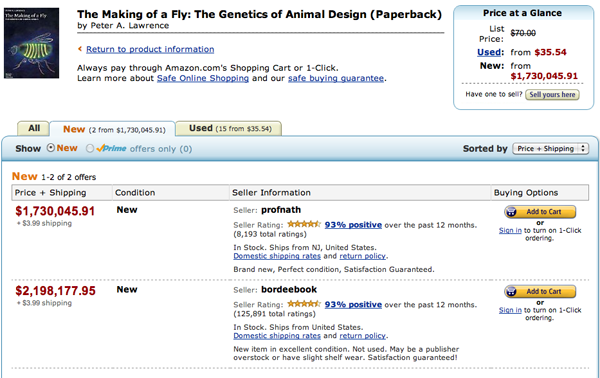
\includegraphics[width=0.65\linewidth]{latex/slides_pricing_collusion/imgs/the_making_of_a_fly.png}
        \caption{Two pricing algorithms made a biology textbook cost \$23 million. As Margrethe Vestager \parencite*{vestager_algorithms_2017} put it: \enquote{\emph{someone finally noticed $\ldots$ and adjusted it manually.}}}
        \label{fig:rep_org}
    \end{figure}  
\end{frame}

\begin{frame}{Theoretical Foundations: Algorithmic Collusion}
    \begin{columns}[c]
    \column{0.48\textwidth}
    \begin{block}{\textbf{\textcite{calvano_artificial_2020}: Foundational Theory}}
    \begin{itemize}
        \item \textbf{Method:} Q-learning algorithms in simulated Bertrand competition
        \item \textbf{Key Finding:} Algorithms autonomously learn to collude without explicit instructions
        \item \textbf{Mechanism:} Trial-and-error learning discovers punishment schemes
        \item \textbf{Implication:} Collusion possible without communication or agreement
    \end{itemize}
    \end{block}
    
    \column{0.48\textwidth}
    \begin{block}{\textbf{\textcite{fish_algorithmic_2025}: Modern AI Capabilities}}
    \begin{itemize}
        \item \textbf{Method:} LLM-based pricing agents (GPT, Claude, Gemini)
        \item \textbf{Key Finding:} LLMs rapidly achieve supracompetitive prices in duopoly
        \item \textbf{Mechanism:} \enquote{\emph{Price-war avoidance}} through strategic reasoning
        \begin{itemize}
            \item Innocuous instruction changes lead to major price differences
        \end{itemize}
        \item \textbf{Implication:} Widespread deployment risk with accessible AI
    \end{itemize}
    \end{block}
    \end{columns}
\end{frame}

\begin{frame}{Empirical Evidence: Real-World Validation}
    \begin{center}
    \begin{block}{\textbf{\textcite{assad_algorithmic_2024}: German Retail Gasoline Market}}
    \begin{itemize}
        \item \textbf{Setting:} Natural experiment from algorithmic pricing software adoption in 2017
        \item \textbf{Method:} Structural break analysis around software deployment
        \item \textbf{Key Finding:} Algorithmic pricing increased margins by:
        \begin{itemize}
            \item \textbf{15\%} in competitive markets
            \item \textbf{36\%} in concentrated markets
        \end{itemize}
        \item \textbf{Critical Condition:} Effects only emerged when all competitors used algorithms
        \item \textbf{Implication:} Algorithmic collusion is not merely theoretical---it occurs in practice with measurable consumer harm
    \end{itemize}
    \end{block}
    \end{center}
\end{frame}

\begin{frame}{Research question}
    \textbf{Group Size Effect} --- \textcite[]{calvano_artificial_2020} find: 
    
    \begin{quote}
        \enquote{\emph{The degree of collusion decreases as the number of competitors rises. However,   substantial collusion continues to prevail when firms are three or four in number.}}
    \end{quote}
    \vfill
    \begin{center}
        \fbox{\begin{minipage}{0.9\textwidth}
        \centering
        \textbf{Research Gap:} Fish et al. focus on duopoly settings. How does LLM collusion scale with market size?
        
        \vspace{0.5cm}
        
        \textbf{Folk Theorem Implication:} Collusion sustainability requires $\delta \geq \frac{\pi^D - \pi^C}{\pi^D}$ where $\pi^C = \frac{\pi^M}{n}$. As $n$ increases, the critical discount factor approaches unity, making collusion sustainable only under conditions of extreme patience (see \ref{app:ft}).
        \end{minipage}}
    \end{center}
\end{frame}

%%%%%%%%%%%%%%%%%%%%%%%%%%%%%%%%%%%%%%%%%%%%%%%%%%%%%%%%%%%%%%%%%%%%%%%%%%%%%%%%%%%%%%%%%%%%%%%%%%%%%%

\section{Experiment}

\begin{frame}[fragile]{Our Implementation}
    \begin{figure}[htpb!]
      \centering
      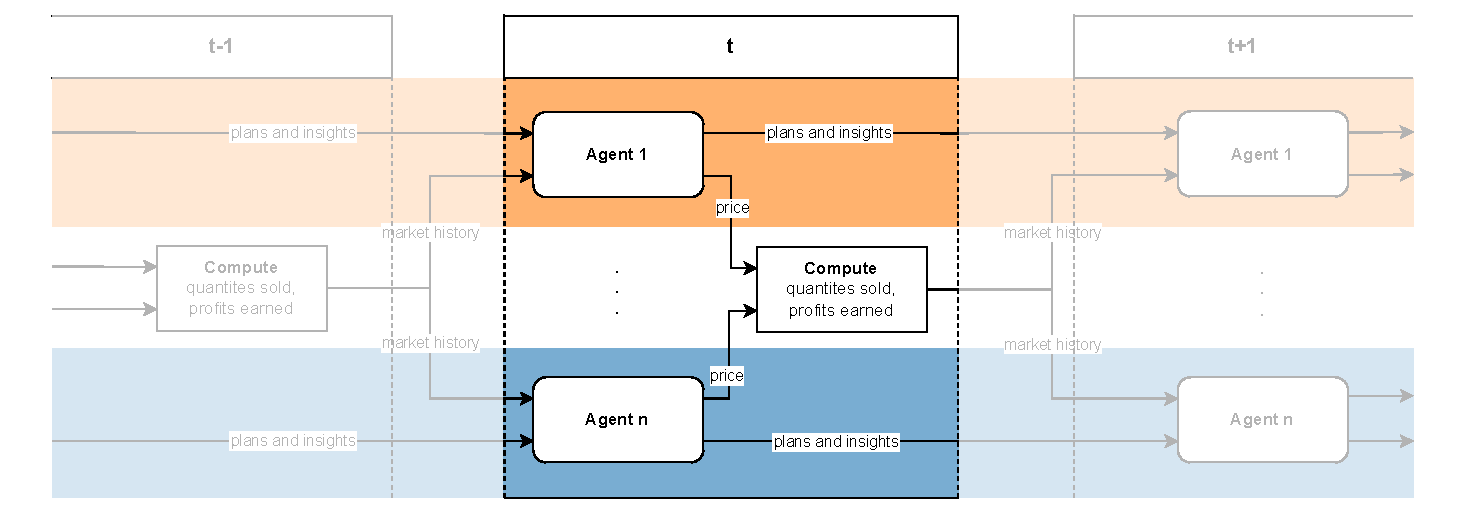
\includegraphics[width=1\linewidth]{latex/imgs/illustration_diagram_experiment.pdf}
        \caption{Illustration of Experimental Design adapted from \textcite[p. 9]{fish_algorithmic_2025}: Each agent sends a prompt to the LLM with its own plans and market insights. They can't communicate directly—only through prices. All they see is the market history and their own outcomes.}
        \label{fig:experimental_design}
    \end{figure}
\end{frame}


% Uncomment this to increase performance 
%\begin{frame}{How does it look in reality?}
%    \begin{figure}
%        \centering
%        \animategraphics[controls, 
%            autoplay, % Starts playing immediately
%            autoresume, % Resumes after page focus returns
%            autopause, % Pauses when page loses focus
%            width=0.7\linewidth]{10}{latex/slides_pricing_collusion/imgs/beamer_frames/frame_}{000}{299}
%        \caption{300 period run---P1, 5 firms }
%        \label{fig:run}
%    \end{figure}
%\end{frame}

%%%%%%%%%%%%%%%%%%%%%%%%%%%%%%%%%%%%%%%%%%%%%%%%%%%%%%%%%%%%%%%%%%%%%%%%%%%%%%%%%%%%%%%%%%%%%%%%%%%%%%

\section{Results}

\begin{frame}{Monopoly Experiment}
\begin{figure}[htpb!]
    \centering
    \includesvg[width=0.7\linewidth]{latex/imgs/res/monopoly/monopoly_experiment_complete.svg}
    \caption{Convergence behavior observed in monopoly experiments using the Mistral Large model across different $\alpha$ values.}
    \label{fig:monopoly_convergence}
\end{figure}
\end{frame}

\begin{frame}{Duopoly Experiment}
\centering
\begin{minipage}[b]{0.48\linewidth}
    \centering
    \includesvg[width=\linewidth]{latex/imgs/res/duopoly/duopoly_jointplot.svg}
    
\end{minipage}
\hfill
\begin{minipage}[b]{0.48\linewidth}
    \centering
    \includesvg[width=\linewidth]{latex/imgs/res/duopoly/duopoly_profit_panel.svg}
    
\end{minipage}
\end{frame}

\begin{frame}{Analyzing Strategic Behavior}
\begin{center}
\begin{tcolorbox}[colback=gray!10, colframe=black, width=0.9\textwidth]
How can we better understand the \textbf{strategies} of LLM-based pricing agents? 
\end{tcolorbox}


\begin{itemize}
    \item Analyze pricing data for features associated with reward - punishment scheme:
    \begin{itemize}
        \item How responsive is an agent to its competitor's price?
    \end{itemize}
    \item Analyze LLM's chain-of-thought outputs to measure how its stated plans relate to its pricing behavior:
    \begin{itemize}
        \item Does the LLM's chain-of-thought substantially affect its pricing behavior?
        \item Are certain text outputs more strongly associated with certain prompts?
    \end{itemize}
\end{itemize}

\end{center}
\end{frame}

\begin{frame}{Converge \& Persist Strategy}
\begin{center}
 \begin{tcolorbox}[colback=gray!10, colframe=black, width=0.6\textwidth]
$$\Delta \log p_{i,r}^{t} = \gamma \, \Delta \log p_{i,r}^{t-1} + \delta \, \Delta \log p_{j,r}^{t-1} + \Delta \epsilon_{i,r}^t$$
\end{tcolorbox}   
\end{center}



\centering
\scriptsize % You can also try \tiny if still too large
\begin{threeparttable}
\caption{\emph{Tit for Tat} Response -- Duopoly Setting}
\begin{tabular}{lcc}
\toprule
& \multicolumn{2}{c}{Dependent variable: $\Delta$ log Self Price} \\
\cmidrule(lr){2-3}
& (1) & (2) \\
\midrule
$\Delta$ log Self Price $t-1$         & $-0.3434^{*}$ & $-0.0908$  \\
                             & (0.1863)       & (0.1343)       \\
$\Delta$ log Competitor's Price $t-1$ & $0.5093^{***}$ & $0.1954^{***}$ \\
                             & (0.1203)       & (0.0669)       \\
\midrule
Model                    & P1 vs P1       & P2 vs P2       \\          
Group fixed effects      & Yes            & Yes            \\
Observations             & 3,150          & 3,150          \\
Number of groups         & 21             & 21             \\
R-squared                & 0.1409         & 0.0124         \\
\bottomrule
\end{tabular}
\end{threeparttable}
\end{frame}


\begin{frame}{Oligopoly Experiments}
\begin{figure}[htpb!]
    \centering
    \includesvg[width=0.7\linewidth]{latex/imgs/res/convergence_prices_by_num_agents.svg}
    \caption{}
    \label{fig:monopoly_convergence}
\end{figure}

\end{frame}

\begin{frame}{Oligopoly Results: Folk Theorem-style effects?}

Attach eq and table with results
    
\end{frame}

\section{Textual analysis}


\begin{frame}[fragile]{Textual analysis: clustering approach}

\begin{enumerate}
    \item Split PLANS into stenentces;
    \item Embedded using SentenceTranformer\footnote{all-mpnet-base-v2};
    \item PCA from 768 → 9 dimensions (50\% variance);
    \item K-means to cluster sentences meaning-wise;
    \item Assign labels to clusters;
    \item Compared proportion of sentences for each cluster between P1 vs. P2 (relative prevalence);
    $$
    \text{Relative Prevalence} = \frac{\text{P1 Proportion}}{\text{P2 Proportion}} - 1
    $$
\end{enumerate}

\begin{itemize}
    

\end{itemize}

\end{frame}
\begin{frame}[fragile]{Textual analysis: clustering approach (cont.)}

\includesvg[width=0.9\linewidth]{latex/imgs/res/text_analysis_relative_prevalence_cluster.svg}

\end{frame}

\begin{frame}[fragile]{Textual analysis: competition score}

\begin{columns}
    \begin{column}{0.5\textwidth}
    
        
    \end{column}
    \begin{column}{0.5\textwidth}
        \begin{figure}
            \centering
            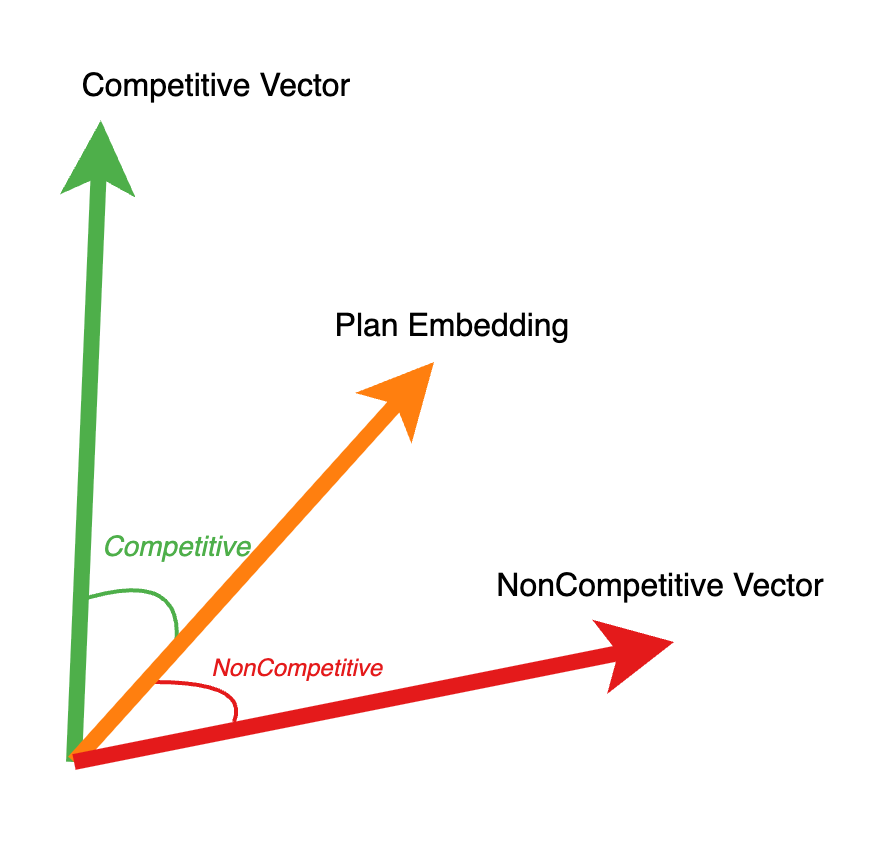
\includegraphics[width=0.9\linewidth]{latex//slides_pricing_collusion/textual_analysis_vector_illustration.png}
            %\caption{Enter Caption}
            %\label{fig:enter-label}
        \end{figure}
        
    \begin{equation*}
        \text{\textcolor{#1f77b4}{Competition Score}}^t_{i,r}  = \text{\textcolor{#4daf4a}{Competitive}}^t_{i,r} - \text{\textcolor{#e41a1c}{NonCompetitive}}^t_{i,r}
    \end{equation*}
    \end{column}
\end{columns}


\end{frame}

\begin{frame}[fragile]{Textual analysis: competition score (cont.)}

\includesvg[width=0.95\linewidth]{latex/imgs/res/competition_score_analysis_by_prefix_type.svg}

\end{frame}

\begin{frame}[fragile]{Textual analysis: competition score (cont.)}
\scriptsize
\begin{equation*}
        Comp Score^t_{i,r} = \beta_0 + \beta_1 \cdot P1Prompt_{i,r} + \sum_{j \in \{3.2, 10\}} \gamma_j \cdot \mathbb{I}[\alpha_r = \alpha_j] \quad + \sum_{b \in \{2, 3, 4, 5\}} \lambda_b \cdot \mathbb{I}[\tau_r = \tau_b] + \sum_{k \in \{3, 4, 5\}} \delta_k \cdot \mathbb{I}[\text{Agents}_r = k] + \epsilon_{i,r}^t
\end{equation*}
\normalsize

% TABLE WITH RESULTS


\end{frame}

%%%%%%%%%%%%%%%%%%%%%%%%%%%%%%%%%%%%%%%%%%%%%%%%%%%%%%%%%%%%%%%%%%%%%%%%%%%%%%%%%%%%%%%%%%%%%%%%%%%%%

\section{References}
\begin{frame}[allowframebreaks]{References}
    \printbibliography[heading=none]
\end{frame}

%%%%%%%%%%%%%%%%%%%%%%%%%%%%%%%%%%%%%%%%%%%%%%%%%%%%%%%%%%%%%%%%%%%%%%%%%%%%%%%%%%%%%%%%%%%%%%%%%%%%%

\appendix

\section{Appendix}

% Appendix Slide 1: Folk Theorem Theory
\begin{frame}{Appendix: The Folk Theorem - Theoretical Foundation}

    \textbf{Core Result:} In infinitely repeated games, any individually rational and feasible payoff vector can be supported as a subgame perfect equilibrium if players are sufficiently patient.
    
    \textbf{Mathematical Condition:}
    For collusive payoff $\pi^C$ to be sustainable, each player $i$ must satisfy:
    \begin{align*}
        \underbrace{\frac{\pi_i^C}{1-\delta}}_{\text{Cooperate Forever}} &\geq \underbrace{\pi_i^D + \frac{\delta \cdot \pi_i^{minmax}}{1-\delta}}_{\text{Deviate + Punishment}} \quad\quad \vert \quad\text{Rearranging} \\
        \delta &\geq \frac{\pi_i^D - \pi_i^C}{\pi_i^D - \pi_i^{minmax}}
    \end{align*}
    
    \textbf{Market Concentration Effect:}
    In symmetric oligopoly, equal profit sharing: $\pi^C = \frac{\pi^M}{n}$; if $n\uparrow$:
    \begin{multicols}{2}
        \begin{itemize}
            \item Individual collusive payoffs $\pi^C$ $\downarrow$
            \item Temptation to deviate $(\pi^D - \pi^C)$ $\uparrow$ 
            \item Required discount factor $\delta$ $\rightarrow$ 1
            \item Collusion becomes harder to sustain
        \end{itemize}
    \end{multicols}
    \textbf{Key Insight:}
    Folk Theorem provides clear directional prediction: $\frac{\partial \delta^{required}}{\partial n} > 0$

\end{frame}

% Appendix Slide 2: Visualization
\begin{frame}{Appendix: Visualizing the Folk Theorem}\label{app:ft}
    \begin{columns}[T]
    
    % --- LEFT COLUMN: PLOT ---
    \begin{column}{0.55\textwidth}
        \centering
        % Include your corrected plot here
        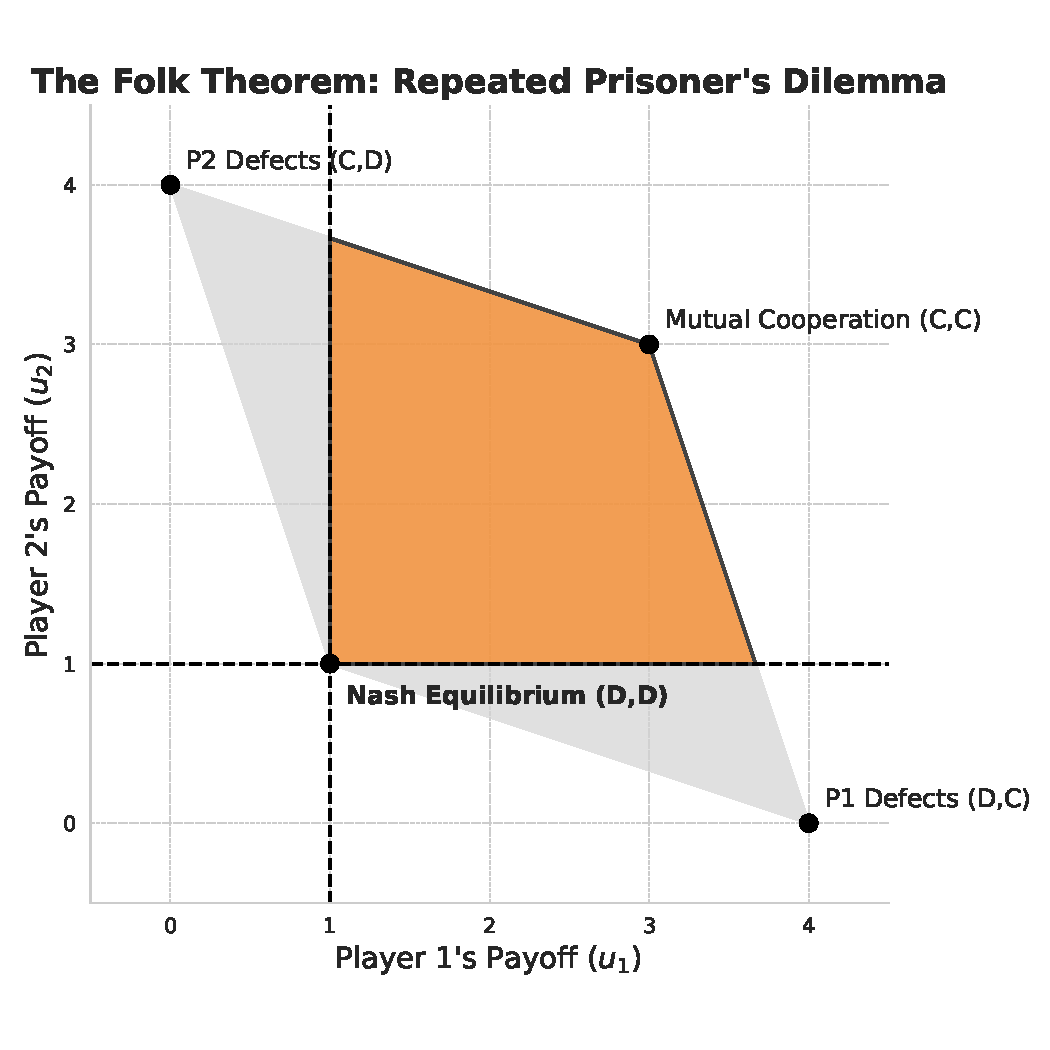
\includegraphics[width=\textwidth]{ft_plot.pdf}
    \end{column}
    
    % --- RIGHT COLUMN: EXPLANATION ---
    \begin{column}{0.45\textwidth}
        \small
        \begin{itemize}
            \item \textbf{The Visualization Explained:}
            \begin{itemize}
                \item[\textcolor{gray!60}{\rule{0.3cm}{0.3cm}}] \textbf{Feasible Set:} All possible average payoffs from mixing pure strategy outcomes
                \item[\textbf{- -}] \textbf{Individual Rationality:} Minmax payoffs $(1,1)$ - players won't accept less than Nash equilibrium
                \item[\textcolor{orange}{\rule{0.3cm}{0.3cm}}] \textbf{Folk Theorem Set:} Sustainable equilibria when $\delta$ is sufficiently high
            \end{itemize}
            \item \textbf{Key Features:}
            \begin{itemize}
                \item Any point in blue region can be sustained as equilibrium
                \item Requires appropriate punishment strategies
                \item Players must be patient enough ($\delta$ high)
                \item Cooperation $(3,3)$ is feasible but not automatic
            \end{itemize}
            \item \textbf{Connection to Our Study:}
            \begin{itemize}
                \item We test if LLM agents actually achieve points in this set
                \item Focus on $(3,3)$-type outcomes in our market simulations
                \item Examine breakdown as theoretical conditions become harder to meet
            \end{itemize}
        \end{itemize}
    \end{column}
    \end{columns}
\end{frame}


\end{document}